\documentclass{ceel}

% ===========================
%Coloque aqui pacotes adicionais, se necessário
\usepackage{hyperref}
\usepackage{verbatim}
\usepackage{array}
%%===========================

% Dados do trabalho
\title{Análise Físico-química e Fundamentos Matemáticos de um Memristor}

\author[1]{\underline{Lesly Viviane Montúfar Berrios}\thanks{leslymontufar@ufu.br}}
\author[1]{Cibelly Cristina Rodrigues Couto\thanks{cibelly.cris@ufu.br}}
\author[1]{Yasmin Delbany Cury\thanks{yasmin.cury@ufu.br}}
\author[2]{Paulo Henrique Oliveira Rezende\thanks{paulohenrique.rezende@ufu.br}}

\affil[1]{FEELT - Universidade Federal de Uberlândia}
\affil[2]{FEELT - Professor Adjunto - Universidade Federal de Uberlândia}

\begin{document}

\inserirtitulo

\begin{multicols}{2}

\textbf{\emph{Resumo} - O objetivo do artigo é estudar o comportamento do quarto elemento de circuito fundamental idealizado por Leon Chua em 1971. Denominado de memristor, sua propriedade de memorizar o último valor de resistência após cessar a passagem de corrente permite aplicá-lo em diversos contextos, como nas memórias ReRam e inteligência artificial.}
\vspace*{10pt}

\textbf{\emph{Palavras-Chave} - Inteligência Artificial, Memórias ReRam, Memristor.}


\begin{center}

%Insira aqui o Título do trabalho em inglês
\noindent\textbf{\large \uppercase{Physicochemical Analysis and Mathematical Foundations of a Memristor}}
\end{center}

\textbf{\emph{Abstract} - The paper purpose is to study the behavior of the fourth fundamental circuit element idealized by Leon Chua in 1971. Called memristor, his property of memorizing the last resistance value after the current flow ceases allows applications in various contexts, as in ReRam memories and artificial intelligence.}
\vspace*{10pt}

\textbf{\emph{Keywords} - Artificial Intelligence, Memristor, ReRam memories.}


\section{Introdução}
%% completar com a palestra de R. Stanley Williams
A teoria de circuitos elétricos abrangia, 150 anos atrás, basicamente três componentes passivos fundamentais: o capacitor (1745), o resistor (1827) e o indutor (1831). No entanto, o professor phD da Universidade da Califórnia, Leon Chua, teve novas considerações a partir da análise de possíveis combinações entre as quatro variáveis fundamentais de circuitos: corrente elétrica $i$, tensão elétrica $v$, carga $q$ e fluxo magnético $\phi$ – sendo as duas últimas descritas como integrais no tempo da corrente e da tensão respectivamente.

Chua observou que o capacitor é definido pela relação entre carga $q(t)$ e tensão $v(t)$ via $qd=C dv$. Similarmente, o resistor pela relação entre a corrente $i(t)$ e tensão $v(t)$ via $dv=R di$, e o indutor pela relação entre o fluxo magnético $\phi(t)$ e a corrente $i(t)$ via $d\phi(t)=L di$. Teria-se então que a combinação das quatro variáveis fundamentais de circuitos resultaria em somente três componentes fundamentais passivos. Assim, baseando-se no argumento de simetria, o estudioso postulou que haveria um elemento de circuito faltante capaz de associar a carga $q(t)$ e o fluxo magnético $\phi(t)$. Sob essa conjectura, em 1971 publicou um artigo no qual idealiza um novo componente por intermédio de demonstrações matemáticas e definido pela relação $d\phi=M dq$, o qual denominou de \emph{memristor}, uma contração de \emph{memory resistor} \cite{artigo}. 

Então considerado o quarto elemento fundamental dos circuitos eletrônicos, ao lado do capacitor, resistor e indutor, o \emph{memristor} destaca-se por apresentar uma propriedade peculiar que o torna promissor em aplicações. Assim como um resistor não-linear, seria definido como um componente eletrônico passivo de duplo terminal utilizado para limitar a corrente em um circuito e dissipar energia térmica, mas também essa limitação, chamada de resistência ou impedância, para o \emph{memristor}, além de se alterar conforme a quantidade de carga elétrica que flui em si, manteria a última resistência obtida até a aplicação de uma nova carga.

Apesar da proposta teórica do \emph{memristor} ter sido apresentada por Chua em 1971, sua primeira implementação prática ocorreu apenas em 2008, nos Laboratórios da Hewllet-Packard (HP), pela equipe liderada pelo físico químico Dr. Richard Stanley Williams. A demora deve-se, principalmente, à inexistência de materiais criação de circuitos, até então, que fossem capazes de conferir a propriedade de reter memória ao dispositivo.

Dessa forma, o componente recentemente sintetizado apresenta a propriedade da não-volatilidade, que, aliada a possibilidade de ser trabalhado em escala nanométrica, garante sua participação na Lei de Moore e expande a aplicabilidade em inúmeraos setores.
Pissardini \cite{memcomputacao} atenta para aplicações de memelementos na elaboração de novas arquiteturas, que, corroborado pelos ideais da Arquitetura de Von Neumann, são capazes de realizar tarefas específicas. 
%% que tarefas? não sei

\begin{comment}
Simulações computacionais representam uma maneira conveniente de estudar circuitos memresistivos. Desse modo, um quadro geral para modelagem de sistemas memristivos, memcapacitivos e memindutivos na família de simuladores SPICE foi proposto em \cite{cibelly1}.
	
A primeira geração de modelos  memristor é baseada em aproximação da dinâmica dos memristores HP TiO2 introduzida em \cite{cibelly2}, entretanto, esses modelos são populares por sua simplicidade, mas sua linear característica estática não é adequada para dispositivos reais. O termo “estática” refere-se a um memristor com variável (s) de estado “congelada”.
\end{comment}

%% mais um paragrafo de aplicacoes:
%% circuitos lógicos CMOS
%% voice encryption - drive
%% memória ReRam !!
%% Computacao neuromorfica, AI, redes neurais CNN

Sob essa perspectiva, a temática deste artigo basear-se-á na descrição detalhada desse novo componente, no âmbito físico, químico e eletrônico, com intuito de compreender o mecanismo interno que atribui propriedades ao \emph{memristor}. É de interesse ainda discutir acerca de algumas das aplicabilidades do dispositivo, para assim poder expor o impacto de sua descoberta para a teoria de circuitos e para o crescimento tecnológico.
%% se formos acrescentar mais alguma coisa como circuito LTSpice.
%% depende das aplicacoes

Na Seção \ref{funcionamento-estrutural} é apresentado o funcionamento estrutural do \emph{memristor} no sentido físico químico. Para, na Seção \ref{analise-matematica}, analisá-lo matematicamente e, assim, provar a natureza de suas propriedades a partir do equaciomento e ilustração gráfica. Finalmente, na Seção \ref{aplicacoes}, é explicitada algumas de suas aplicações e recentes estudos.


%% precisa colocar imagem pequena para explicar que a propriedade do memristor deve-se basicamente à redistribuição das lacunas(+) devido à deficiencia em oxigenio.
%% de preferencia a msm imagem do R. Stanley Williams
\section{Funcionamento estrutural de um memristor} \label{funcionamento-estrutural}
Dispositivos constituídos por óxidos com a capacidade de mudar o valor de resistência, %% existe algum dispositivo constuido por óxido que mude outra grandeza? qual? (apresentação)
assim como os \emph{memristores}, são bastante úteis para diversos processos, pois %% ?
admitem as características de operação em baixas tensões, alta velocidade e densidade, %% ?
assim como a não-volatilidade \cite{conceito}, o que significa que o dispositivo possui determinada estabilidade no armazenamento do valor da última resistência obtida. 

A fim de cumprir tais características e funções no circuito, o memristor deve ser construído de maneira específica. A estrutura de um dispositivo memristor, basicamente, possui dois eletrodos entre os quais existe uma área isolante, porém com uma nanopartícula que fornece um caminho condutivo entre os eletrodos. %% continuar essa parte
%% aqui comeca assunto diferente, pode ficar para o final da seção
Um memristor pode compreender diversos materiais, sendo os mais utilizados materiais óxidos, geralmente de titânio ou tântalo \cite{us} ($TiO_x$, $TaO_x$).

O funcionamento molecular de um memristor é baseado no movimento de íons livres no meio dielétrico (óxido), o que torna possível o comportamento “memristivo” pois cria mudanças locais na condutividade, causando, assim, a modelagem de filamentos condutores entre os eletrodos. \cite{us}. %% essa é a continuação

Para a formação de tais filamentos condutores entre os eletrodos no meio inicialmente dielétrico (meio entre os dois eletrodos), é necessário realizar um processo conhecido, em inglês, como “electroforming”, ou “eletroformação”. Tal %% o electroforming está na patente?
processo consiste em aplicar uma tensão elétrica suficientemente alta, ou seja, um valor limite, entre os dois eletrodos por um período de tempo suficiente para ser originado um canal condutivo local no meio isolante. O que ocorre é, basicamente, o rompimento da rigidez dielétrica do material que permanece entre os eletrodos. %% explicacao do electrofoming terminou
Os valores limite de tensão e de tempo necessários para ser formado o canal condutivo dependem de qual dielétrico foi utilizado e do material do qual são formados os dois eletrodos, além da estrutura geométrica do dispositivo \cite{us}.Consequentemente, é possível formar diferentes “status” do memristor, como “OFF”, ou seja, um estado de alta resistência; “ON”, ou seja, um estado de baixa resistência, e ainda estados intermediários. %% armazena dados em multinível e não apenas na forma binária. MLC? 
%% Multi Layer Cell ou, traduzindo, Células de Múltiplas Camadas. Esse é o significado de MLC. Aqui, cada célula de memória é capaz de armazenar dois bits em vez de apenas um: 00, 01, 10 ou 11.
%% memórias MLC são muito usadas em SSDs para computadores domésticos.

Para analisar o funcionamento prático de um memristor, pode-se analisar o funcionamento prático de um dispositivo que foi a base para a existência do memristor, o "crossbarlatch", estudado em 2006 pelos %% volta no tempo, poderia colocar essa parte mais para o inicio antes do electroforming
laboratórios da HP. Tal dispositivo passou a ser conhecido como o próprio memristor posteriormente. O "crossbarlatch" era uma espécie de sanduíche, possuindo suas partes externas constituídas por Platina(Pt), com espessura inferior a 3 nanômetros, e sua camada intermediária sendo dividida em duas partes, sendo a primeira formada de óxido de titânio($TiO_2$) e a segunda formada pela mesma substânica, porém deficiente em oxigênio ($TiO_2-x$) \cite{construcao}.  

A parte constituída por $TiO_2$ é conhecida como a parte pura(ou não dopada) e a parte deficiente em oxigênio é conhecida como a parte dopada. Ao se aplicar uma tensão elétrica positiva no terminal dopado, as lacunas (onde falta oxigênio) se comportam como cargas positivas e "migram" para o outro lado, ou seja, cargas negativas se deslocam para a parte dopada. Dessa forma, a espessura da camada intermediária diminui, ao mesmo tempo que a espessura da camada condutora aumenta, o que resulta na diminuição do valor da resistência do dispositivo. Tal estado do memristor é conhecido como "ON", ou baixa resistência. %% Stanley fala isso na palestra, procurar documento que tem oq ele diz na forma de artigo fácil de entender

Por outro lado, ao se aplicar uma tensão negativa no terminal dopado, as lacunas são "atraídas", ou seja, a espessura da camada intermediária aumenta, ao mesmo tempo que a espessura da camada condutora diminui, causando um aumento no valor da resistência do memristor. Tal estado é conhecido como "OFF", ou alta resistência. 

Ainda pode-se analisar o comportamento do memristor nos momentos em que não há aplicação de tensão elétrica, ou seja, quando a fonte de alimentação for desligada. Nesta situação, as camadas pura e dopada permanecem no mesmo estado que estavam anteriormente. Assim, no momento em que uma tensão for aplicada, a memristência começa do ponto em que tinha estacionado antes. %% no momento == quando

Assim, o princípio básico do funcionamento de um memristor é a mudança de posição dos átomos quando sofre influência de uma tensão elétrica, processo que é facilitado por ocorrer em escala nanométrica. %% por que?

\section{Análise Matemática}\label{analise-matematica}
O \emph{memristor}, a princípio, foi definido por Chua pela relação $d\phi=M dq$, equivalentemente tem-se $v=M(q)i$, do que se conclui que a \emph{memristência} $M$ é mensurada na mesma unidade que a resistência. Entretanto, a simples relação é incapaz de descrever o dispositivo completamente, diante disso, a equipe HP Laboratories decidiu que essencialmente seriam necessárias duas equações para descrevê-lo: Equações \ref{eq01} e \ref{eq02}, sendo que a Equação \ref{eq02} envolve o aspecto físico do componente, já apresentado na Seção \ref{funcionamento-estrutural}.

\begin{equation}\label{eq01}
v=M( w) \ i
\end{equation}

\begin{equation}\label{eq02}
\dfrac{dw}{dt} =f(i) 
\end{equation}

Assim, a definição matemática rigorosa revela que a \emph{memristência} $M$ depende da variável estática $w$, que por sua vez referencia-se na função contínua de corrente $f$.
%% Lisajous Figures


\begin{minipage}[h]{\columnwidth}
\centering
\captionsetup{type=figure}
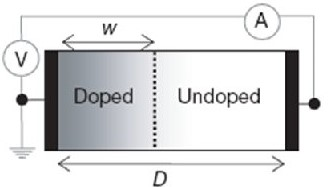
\includegraphics[width=0.8\columnwidth]{memristor004}
\caption{Memristor}\label{memristor}
\end{minipage}

\section{Aplicações}\label{aplicacoes}
\subsection{Mémorias ReRam}
A Memória Resistiva de Acesso Randômico (ReRAM), assim como a memória de acesso aleatório magnéticas (MRAM), mantêm os dados na falta de energia, essa propriedade deve-se especialmente pela presença do memristor em seus chips, que altera sua resistência à passagem da corrente elétrica em resposta a variações na sua tensão de alimentação.
Essa tecnologia assemelha ao uso de transistores nas memórias Flash, com a diferença de as células de memória ReRAM poderem ser muito menores, consumir menos energia elétrica e ter desempenho para leitura e escrita de dados próximos aos de módulos da Memória de Acesso Randômico Dinâmica (DRAM)\cite{blog} , que diferentemente da memória ReRAM (que armazena os dados como resistência), essa armazena os dados como carga elétrica.
O reRAM, portanto, tem o potencial de ser extremamente denso, de baixa potência, com alta resistência, tornando-se uma tecnologia atraente para armazenamento secundário e níveis de memória de classe de armazenamento \cite{prog}. Segundo a HP, dispositivos contendo memristores oferecem em média algo em torno de 20GB por centímetro quadrado, o dobro da capacidade projetada para as memórias flash \cite{hp}.
Dispositivos memresistivos podem mudar o paradigma padrão da computação ao permitir que cálculos sejam executados nos chips onde a informação está armazenada \cite{hp}. Além disso, essa tecnologia é passível de utilização em todo o tipo de dispositivo, desde celulares e MP3 players, que primariamente utilizam memórias flash NAND, como SSD (solid state disk, as memórias flash) e DRAM.

\subsection{Circuitos Lógicos}



\section{CONCLUSÕES}


%==================================
% REFERÊNCIAS
%==================================
\begin{thebibliography}{9}

%% INTRODUCAO
\bibitem{memcomputacao}
    R. S. Pissardini,
    “MEMCOMPUTAÇÃO: CARACTERÍSTICAS E APLICAÇÕES EM
COMPUTAÇÃO PARALELA”, Escola Politécnica da Universidade de São Paulo, Departamento de Engenharia de Transportes, Laboratório de Topografia e Geodesia.
 Disponível em:
 \url{https://www.ime.usp.br/~gold/cursos/2015/MAC5742/reports/MemComputacao.pdf}. Acesso em: jun. 2019.

\bibitem{artigo}	
    L. Chua,
    “Memristor - the missing circuit element”, 
    in \emph{IEEE Transactions on circuit theory}, VOL. CT-18, NO. 5, Setembro 1971.
    
\begin{comment}
\bibitem{cibelly1}	
    D. Biolek, Z. Biolek, and V. Biolková, “\uppercase{SPICE modeling of memristive,
    memcapacitative and meminductive systems},” in Proc. of the European
    Conference on Circuit Theory and Design (ECCTD09), Antalya,
    Turkey, 2009, pp. 249-252. %% ainda não

\bibitem{cibelly2}	
    D. B. Strukov, G. S. Snider, D. R. Stewart, and R. S. Williams, “\uppercase{The
    missing memristor found}”, Nature, 2008, vol. 453, pp. 80–83. %% preciso baixar esse artigo
\end{comment}

%% FUNCIONAMENTO ESTRUTURAL
\bibitem{conceito}	
    J. P. Strachan, A. C. Torrezan, F. Miao, M. D. Pickett, J. J. Yang; W. Yi, G. M. Ribeiro, R. S. Williams, “STATE DYNAMICS AND MODELING OF TANTALUM OXIDE MEMRISTORS”, Disponível em: \url{https://ieeexplore.ieee.org/stamp/stamp.jsp?arnumber=6542012}. Acesso em ago. 2019.
    
\bibitem{us}	
    United States Patent; Patent No: US 9035272 B2. “NANOPARTICLE-BASED MEMRISTOR STRUCTURE”. Disponível em: \url{https://patentimages.storage.googleapis.com/0e/70/e0/6b8926f49e7cd8/US9035272.pdf}. Acesso em ago. 2019.
    
\bibitem{construcao}	
   F.S.Barachati, "ESTUDO E PREPARAÇÃO DE MEMORISTORES PARA SUA APLICAÇÃO EM DISPOSITIVOS ELETRÔNICOS". Escola de Engenharia de São Carlos, da Universidade de São Paulo. Disponível em: \url{http://www.tcc.sc.usp.br/tce/disponiveis/18/180450/tce-26032012-090929/publico/Barachati_Fabio_Souza.pdf}. 
   Acesso em ago. 2019.

%% MATEMATICA
\bibitem{elusive} % indescritivel
    Y. N. Joglekar, S. J. Wolf, "The elusive memristor: properties of basic electrical circuits", Department of Physics, Indiana University Purdue, 2009.

%% APLICACOES

%% MEMORIAS RERAM
\bibitem{blog}
   E. Alecrim, ”Os primeiros chips ReRAM fabricados em larga escala chegarão em breve”, 2013. Disponível em: \url{https://tecnoblog.net/136874/primeiros-chips-reram-em-larga-escala/}. Acesso em ago. 2019.
   
\bibitem{prog}
    M. Ramadan, N. Wainstein, R. Ginosar, S. Kvatinsky, "Adaptive programming in multi-level cell ReRAM", Microelectronics Journal, Volume 90, 2019. %% MULTI-LEVEL CELL == MLC ?!
    %% bem recente :)
    
\bibitem{hp}
A. Martins, “ReRAM - A próxima geração de memórias e CPU’s”,2010. Disponível em: <https://brainstormdeti.wordpress.com/2010/09/15/reram-\%E2\%80\%93-a-proxima-geracao-de-memorias-e-cpu\%E2\%80\%99s/>. Acesso em ago.2019

%% CIRCUITOS LOGICOS


\end{thebibliography}



\end{multicols}
\end{document}
